% Präambel
\documentclass[11pt,a4paper,oneside, 
liststotoc, 					% Tabellen- und Abbildungsverzeichnis ins Inhaltsverzeichnis
bibtotoc,						% Literaturverzeichnis ins Inhaltsverzeichnis aufnehmen
titlepage, 						% Titlepage-Umgebung statt \maketitle
headsepline, 					% horizontale Linie unter Kolumnentitel
%abstracton,					% Überschrift beim Abstract einschalten, Abstract muss dazu in {abstract}-Umgebung stehen
%DIV11,							% auskommentieren, um den Seitenspiegel zu vergrößern
BCOR6mm,						% Bindekorrektur, die den Seitenspiegel um 6mm nach rechts verschiebt,
]{scrreprt}			
\usepackage{ucs} 				% Dokument in utf8-Codierung schreiben und speichern
\usepackage[utf8x]{inputenc} 	% ermöglicht die direkte Eingabe von Umlauten
\usepackage[ngerman]{babel} 	% deutsche Trennungsregeln und Übersetzung der festcodierten Überschriften
\usepackage[T1]{fontenc} 		% Ausgabe aller zeichen in einer T1-Codierung (wichtig für die Ausgabe von Umlauten!)
\usepackage{graphicx}  			% Einbinden von Grafiken erlauben
%\usepackage{amsmath}
%\usepackage{amsfonts}
%\usepackage{amssymb}
\usepackage{mathpazo} 			% Einstellung der verwendeten Schriftarten
\usepackage{textcomp} 			% zum Einsatz von Eurozeichen u. a. Symbolen
\usepackage{listings}			% Datstellung von Quellcode mit den Umgebungen {lstlisting}, \lstinline und \lstinputlisting
\usepackage{xcolor} 			% einfache Verwendung von Farben in nahezu allen Farbmodellen
\usepackage[intoc]{nomencl} 	% zur Erstellung des Abkürzungsberzeichnisses
\usepackage{fancyhdr}			% Zusatzpaket zur Gestaltung von Fuß und Kopfzeilen
\usepackage{graphicx}
\usepackage{hyperref}
\usepackage[ngerman]{cleveref} 

% -----------------------------------------------------------------------------------------------------------------
% Zum Aktualisieren des Abkürzungsverzeichnisses bitte auf der Kommandozeile folgenden Befehl aufrufen :
%  makeindex Studienarbeit.nlo -s nomencl.ist -o Studienarbeit.nls
% -----------------------------------------------------------------------------------------------------------------

% Hier die persönlichen Daten eingeben:

\newcommand{\titel}{BYOD}
\newcommand{\untertitel}{Konzeptionierung einer Entscheidungsempfehlung für ein mittelständiges Unternehmen}
\newcommand{\arbeit}{Studienarbeit}
\newcommand{\studiengang}{Informationstechnik}
\newcommand{\autor}{Nicolas Konle, Luka Kröger}
\newcommand{\matrikelnr}{MATRIKELNUMMERN}
\newcommand{\kurs}{TINF15B3}
\newcommand{\abgabe}{\today}
\newcommand{\betreuerdhbw}{Ralf Brune}

\newcommand{\jahr}{2018}			% für Angabe im Copyright-Vermerk der Titelseite

% Abkürzungen
\newcommand{\ua}{\mbox{u.\,a.\ }}
\newcommand{\zB}{\mbox{z.\,B.\ }}
\newcommand{\bs}{$\backslash$}

\renewcommand{\nomname}{Abkürzungsverzeichnis}

% -------------------------------------------------------------------------------------------
% Definition der Kopf- und Fußzeilen
\lhead{}								% Kopf links
\chead{}								% Kopf mitte
\rhead{\sffamily{\titel}}				% Kopf rechts
\lfoot{}								% Fuß links
\cfoot{\sffamily{\thepage}}				% Fuß mitte
\rfoot{\sffamily{\autor}}				% Fuß rechts
\renewcommand{\headrulewidth}{0.4pt}	% Liniendicke Kopf
\renewcommand{\footrulewidth}{0.4pt}	% Liniendicke Fuß


\makenomenclature							% Abkürzungsverzeichnis erstellen

% alle Abkürzungen, die in der Studienarbeit verwendet werden

\nomenclature{DHBW}{Duale Hochschule Baden-Württemberg}
\nomenclature{Sem}{Semester}
\nomenclature{OSS}{Open Source Software}					% Datei mit Abkürzungen laden

% -------------------------------------------------------------------------------------------
%                     Beginn des Dokumenteninhalts
% -------------------------------------------------------------------------------------------
\begin{document}
\setcounter{secnumdepth}{3}					% Nummerierungstiefe fürs Inhaltsverzeichnis
\setcounter{tocdepth}{3}
\sffamily									% für die Titelei serifenlose Schrift verwenden

% ------------------------------ Titelei -----------------------------------------------------

\thispagestyle{plain}
\begin{titlepage}
\enlargethispage{4.0cm}
\sffamily 								% Serifenlose Grundschrift für die Titelseite einstellen
				
\begin{flushright}

\includegraphics[scale=2.0]{Bilder/logo_dhbw.jpg}\\[5ex]
\end{flushright}

\begin{center}

\huge{\textsc{\textbf{\titel}}}\\[1.5ex]
\Large{\textbf{\untertitel}}\\[5ex]
\LARGE{\textbf{\arbeit}}\\[2ex]
\normalsize{für die Prüfung zum\\[1ex] Bachelor of Engineering}\\[3ex]
\Large{Studiengang \studiengang}\\[1ex]
\normalsize{Duale Hochschule Baden-Württemberg Karlsruhe}\\[5ex]
von\\[1ex] \autor \\[18ex]


\end{center}

\begin{flushleft}

\begin{tabular}{ll}
Abgabedatum:					& \quad \abgabe \\
Bearbeitungszeitraum:			& \quad 12 Wochen   \\ 
Matrikelnummer, Kurs: 			& \quad \matrikelnr , \kurs \\ 
Betreuer der Dualen Hochschule: & \quad \betreuerdhbw \\ [5ex]

\end{tabular} 



\small
Copyrightvermerk:\\

Dieses Werk einschließlich seiner Teile ist \textbf{urheberrechtlich geschützt}. Jede Verwertung außerhalb der engen Grenzen des Urheberrechtgesetzes ist ohne Zustimmung des Autors unzulässig und strafbar. Das gilt insbesondere für Vervielfältigungen, Übersetzungen, Mikroverfilmungen sowie die Einspeicherung und Verarbeitung in elektronischen Systemen.
\end{flushleft}
\begin{flushright}
\copyright{} \jahr
\end{flushright}
\end{titlepage} 				% erzeugt die Titelseite
\pagenumbering{Roman}						% große, römische Seitenzahlen für Titelei
\addchap{Eidesstattliche Erklärung}
Ich versichere hiermit, dass ich meine Studienarbeit mit dem Thema
\begin{quote}
\textit{\titel} -\textit{ \untertitel }
\end{quote}
selbständig verfasst und keine anderen als die angegebenen Quellen und Hilfsmittel benutzt habe. Die Arbeit wurde bisher keiner anderen Prüfungsbehörde vorgelegt und auch nicht veröffentlicht.


Mir ist bekannt, dass ich meine Diplomarbeit zusammen mit dieser Erklärung fristgemäß nach Vergabe des Themas in dreifacher Ausfertigung und gebunden im Sekretariat meines Studiengangs an der DHBW Karlsruhe abzugeben habe. Als Abgabetermin giltbei postalischer Übersendung der Eingangsstempel der DHBW, also nicht der Poststempel oder der Zeitpunkt eines
Einwurfs in einen Briefkasten der DHBW.\\[10ex]

Karlsruhe, den \today \\[4ex]


\rule[-0.2cm]{5cm}{0.5pt} \\

\textsc{\autor} \\[10ex]

% Sperrvermerk bei Bedarf dekommentieren
\hrule 
\vspace*{1.0cm}
\noindent \textbf{\Large{Sperrvermerk}}\\
\normalsize 				% Einbinden der eidestattlichen Erklärung
\chapter*{Abstract/Zusammenfassung} %*-Variante sorgt dafür, das Abstract nicht im Inhaltsverzeichnis auftaucht

Hier bitte den Abstract Ihrer Arbeit eintragen. Der Abstract sollte nicht länger als eine halbe Seite sein. Bitte klären Sie mit Ihrem Studiengangsleiter ab, ob der Abstract in englischer oder deutscher Sprache (oder möglicherweise sogar in beiden Sprachen) verfasst werden soll.
   				% Einbinden des Abstracts

\tableofcontents							% Erzeugen des Inhalsverzeichnisses
\printnomenclature[2.0cm]					% Erzeugen des Abkürzungsverzeichnisses
\listoffigures 								% Erzeugen des Abbildungsverzeichnisses 
\listoftables 								% Erzeugen des Tabellenverzeichnisses
\pagebreak

% --------------------------------------------------------------------------------------------
%                    Inhalt der Studienarbeit
%---------------------------------------------------------------------------------------------
\pagenumbering{arabic}						% arabische Seitenzahlen für den Hauptteil
\pagestyle{fancy}					
\rmfamily

\chapter{Einleitung}
\label{cha:Einleitung}

\section{Motivation}
\label{sec:Motivation}

\section{Ziel der Arbeit}
\label{sec:ZielDerArbeit}

\section{Aufbau der Arbeit}
\label{sec:AufbauDerArbeit}




\chapter{Ausgangssituation}
\label{cha:Ausgangssituation}
Im Rahmen dieser Studienarbeit wird das fiktive Unternehmen „Loco AG“ als Grundlage für die Konzeptionierung der Entscheidungsempfehlung verwendet, um eine konkrete Ausarbeitung zum Themenbereich „Bring your own Device“ zu geben. Im Folgenden wir das Unternehmen vorgestellt:
Die „Loco AG“ ist ein mittelständiges Unternehmen ansässig in der Architekturbranche mit dem Hauptsitz in Karlsruhe. Das Unternehmen beschäftigt deutschlandweit 450 Mitarbeiter und hat einen jährlichen Umsatz von XXX€.

Das momentane Geschäftsmodell besteht darin, Kunden zu deren Geschäftsstellen zu bestellen und mit Ihnen in betriebseigenen Meetingräumen Geschäfte abzuschließen. Die „Loco AG“ möchte gerne Ihr Unternehmen erweitern und höherwertige Kunden erreichen. Hierbei evaluieren die Geschäftsführer mehrere Optionen für die Expansion: Die erste Variante wäre ein neues  Kundencenter. Als zweite Lösung wäre die Änderung der Geschäftsstrategie auf den Außendienst. Das heißt die Beratung tritt direkt vorort beim Kunden statt. 

Das Unternehmen verwendet eine internentwickelte Architektursoftware, welche Anbindung auf die zentralliegende Datenbank benötigt. Die Entwicklungsabteilung hat bereits eine Version für das Smartphone und Tablet entwickelt, aber es findet noch keine richtige Verwendung.

 





\chapter{Definitionen}
\label{cha:Definitionen}\marginpar{ Alle Texte hier sind von \cite{Air2018}. Also abändern}

\section{Bring Your Own Device}
Bring Your Own Device (BYOD) ist eine IT-Richtlinie, die es Mitarbeitern erlaubt, ihre privaten Geräte für Arbeitszwecke zu verwenden. EMM-Plattformen ermöglichen durch die Trennung von Arbeits- und Privatdaten auf Geräten die Implementierung einer BYOD-Strategie, ohne die Sicherheit oder die Privatsphäre der Mitarbeiter aufs Spiel zu setzen. Durch diese Datentrennung ist die IT in der Lage, auf einem mitarbeitereigenen Gerät ausschließlich Arbeitsdaten zu verwalten und abzusichern. Sobald ein Gerät kompromittiert ist oder ein Mitarbeiter das Unternehmen verlässt, kann die IT lediglich arbeitsbezogene Daten entfernen, ohne dabei private Elemente auf dem Gerät zu beeinflussen. 

\section{Mobile Device Management (MDM)}
Mobile Device Management (MDM) ist eine Technologie zur Lebenszyklusverwaltung, mit der die IT Mobilgeräte durch auf den Geräten installierte MDM-Profile einsetzen, konfigurieren, verwalten, unterstützen und sichern kann. MDM Software ermöglicht Anlageninventur, Over-the-Air-Konfiguration von E-Mail, Anwendungen und WLAN, Remotefehlerbehebung sowie Remotesperr- und Remote Wipe-Funktionen zur Sicherung von Geräten und den darauf befindlichen Unternehmensdaten. MDM ist die Grundlage für eine umfassende Enterprise Mobility Management-Lösung (EMM). 

\section{Mobile Application Management}
Mobile Application Management-Technologien (MAM) wenden Tools der Verwaltungs- und Richtlinienkontrolle auf individuelle Anwendungen statt auf das gesamte Gerät an. Üblicherweise bieten MAM-Lösungen einen benutzerdefinierten App Store, der die Kontrolle und Bereitstellung von sowohl intern entwickelten als auch Drittanbieteranwendungen erlaubt. IT-Administratoren haben die Möglichkeit, mithilfe von AppConfig Community-Standards oder Software Development Kit- oder App Wrapping-Lösungen vom MAM-Anbieter der Anwendung Sicherheits-, Verschlüsselungs- und Kontrollfunktionen hinzuzufügen. 

\section{Mobile Content Management}

\section{Enterprise Mobility Management}
Enterprise Mobility Management (EMM) ist eine geräte- und plattformagnostische Lösung, in der die Verwaltung, Konfiguration und Sicherheit aller Geräte – BYO sowie unternehmenseigenen – einer Organisation zusammengefasst werden. EMM erstreckt sich über traditionelle Geräteverwaltung hinaus auf die Verwaltung und Konfiguration von Unternehmensanwendungen und -inhalten.  Eine solide EMM-Lösung umfasst üblicherweise MDM, MAM, Mobile Content Management (MCM), Identitätsmanagement zur Zugriffskontrolle sowie Produktivitätsanwendungen zum mühelosen Zugriff auf E-Mail, Kalender, Kontakte, Inhalts-Repositorys und Intranet-Sites des Unternehmens. Darüber hinaus sollte eine EMM-Lösung es technisch ermöglichen, der IT die Verwaltung und Sicherheit zu erleichtern und gleichzeitig den Mitarbeitern ein angenehmes Benutzererlebnis zu bieten. 

\section{Unified Endpoint Management}
Mithilfe von Unified Endpoint Management (UEM) ist die IT endlich in der Lage, sich der unterschiedlichen Tools für die Verwaltung von Mobilgeräten, Desktops und seit Kurzem auch IdD-Geräten (Internet der Dinge) zu entledigen. Durch die Kombination von traditioneller Client-Verwaltung von Desktop- und PC-Systemen mit einem modernen Enterprise Mobility Management Framework (EMM) schaffen UEM-Lösungen die Voraussetzung für einen ganzheitlichen und anwenderorientierten Ansatz zur Verwaltung aller Endpunkte. Eine solide UEM-Lösung befähigt die IT zur Verwaltung von Benutzern und zur Realisierung eines einheitlichen Erlebnisses entlang aller Endpunkte sowie zur Sicherung und Verwaltung des gesamten Gerätelebenszyklus – und alles über eine zentrale, umfassende Plattform. 







\chapter{Systeme}
\label{cha:systeme}
Als Entscheidungsgrundlage für die Auswahl der zu vergleichenden "Bring Your Own Device" Lösungen dient das sogenannte "Magic Qadrant" von Gartner. Das Marktforschungsinstitut Gartner nutzt diese Art der Visualisierung um die Positionen verschiedener Unternehmen in einem Technologie-Markt darzustellen.  Hierbei werden die Quadranten in die  Bereiche Niche Players, Visionäre, Challengers und Leader unterteilt. Diese Bewertung dient als erste Filterung der in dieser Studienarbeit verglichenen BYOD Lösungen. Alle nachfolgenden Systeme erreichten die höchsten Punktzahlen um in den Quadranten Leader aufgenommen zu werden (Stand Juni 2016) Samsung Knox wurde von Gartner in dieser Auswertung nicht betrachtet. Aufgrund der hohen Marktanteile von Samsung Endgeräten wurde jedoch entschiedenen diese Lösung auch zu untersuchen. 
Quelle: Gartner Magic Quadrant
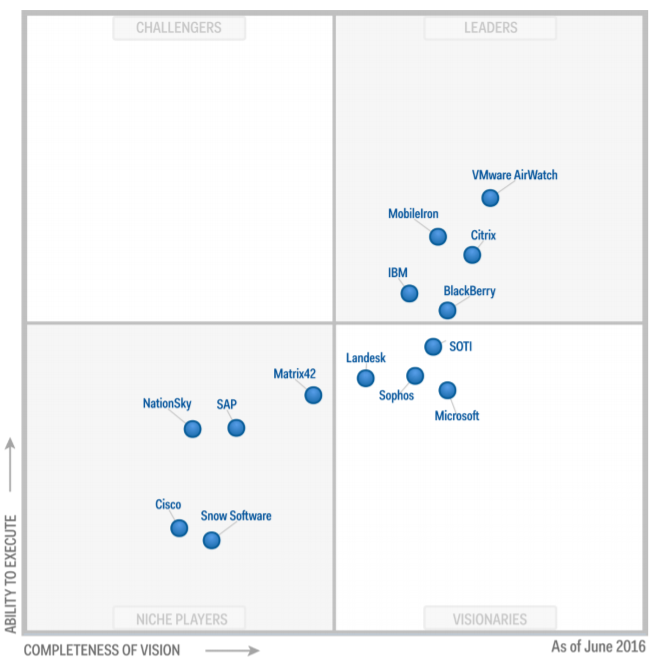
\includegraphics[width=0.75\textwidth]{Bilder/magicq.png} 
\section{MobileIron}

\subsection {Allgemein} 
Das Unternehmen MobileIron ist ein US-amerikanisches Unternehmen mit Hauptsitz in Kalifornien welches im Jahr 2007 gegründet wurde. MobileIron hat sich von Anfang an auf die Verwaltung von mobilen Endgeräten im Enterprise Umfeld spezialisiert. Das Unternehmen wurde 2017 im siebten Jahr in folge als Leader im Magic Quadrant von der Gartner Inc. neben VMWare, IBM und BlackBerry für MDM/EMM Suites gekürt. Das Softwareentwicklungsunternehmen bietet in Ihrem Produktportfolio verschiedene Bring Your Own Device Pakete mit zahlreichen Funktionen an. 
\subsection {Kompatibilität}
Der Hersteller MobileIron unterstützt in seinen Lösungen die  mobilen Endgeräte Apple iOS, Google Android und Microsofts Windows Phone. Zusätzlich können klassische Desktop Geräte mit den Betriebssystemen Microsoft Windows (ab 8.1) und Apple OS X (ab 10.9)  verwaltet werden. 
\subsection {Paketmodelle}
MobileIron bietet die drei verschiedenen Bundles „EMM Silver“, „EMM Gold“ oder „EMM Platinum“ seiner Bring Your Own Device Lösung an.
Das Basispaket „EMM Silver“ beinhaltet die Komponenten „Core“ „Sentry „und „Apps@Work“. Das Paket „EMM Gold“ ist um die Module „Email+“, „Docs@Work“ und „Web@Work“ erweitert. Durch die Wahl des Platinum Pakets ergänzt sich dieses wiederum um „Help@Work“, „Tunnel“, „MobileIron Monitor“ und „ServiceConnect-Integration“.

\begin{figure}[hbt]
\centering
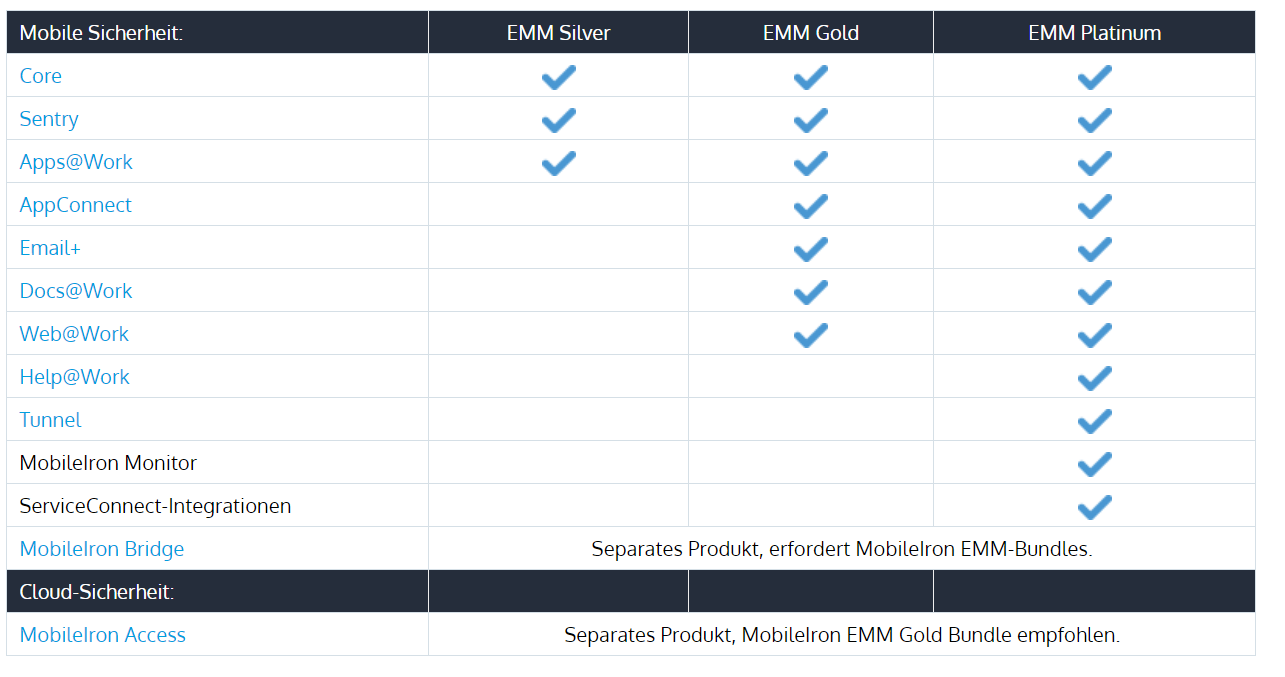
\includegraphics[width=0.95\textwidth]{Bilder/mi_1.png} 
\caption{Mobile Iron Paketmodelle}\label{fig:MobIro1}
\end{figure}

\subsection {Pakete}
\subsubsection {Core}
Das Paket Core ist das zentrale Modul, welches das IT-Backend des Unternehmens einbindet. Hierüber können die erforderlichen Sicherheits- und Verwaltungsrichtlinien der mobilen Endgeräte definiert und verwaltet werden. Über die  API Schnittstellen des Cores kann man komfortabel Erweiterungen nutzen. Im Fokus des Cores stehen jedoch die das MDM, MAM und MCM. Der Core bietet für die Administratoren zusätzliche Analyse- und Auswertungsfunktionen. So kann beispielsweise der von den Endgeräten produzierten Netzwerktraffic ausgewertet werden um Infrastrukturprobleme zu lokalisieren. Durch die Möglichkeit Dachboards-Widgets anzulegen kann der Administrator das System und die verschiedenen Gerätestatus komfortabel überblicken. 
\subsubsection {Sentry}
Die Komponente Sentry ist das Inline-Gateway, das den gesamten Netzwerkverkehr zwischen den Mobilgeräten und dem Unternehmensbackend verschlüsselt, verwaltet und sichert. Sentry setzt die in der Core Komponente definierten Sicherheitsrichtlinien um. Sentry kann beispielsweise E-Mail Anhänge verschlüsseln, sodass nicht autorisierte Applikationen auf diese Daten nicht zugreifen können. 

\subsubsection {Apps@Work}
Apps@Work ist ein unternehmenseigener App Store, indem sowohl eigenentwickelte als auch öffentliche, freigegebene Anwendungen für die Benutzer bereitgestellt werden können. Über diesen Weg können Administratoren schnell auswählen, welche Anwendungen erforderlich, zulässig oder verboten sind. 
\subsubsection {AppConnect}
Durch AppConnect können auf den Endgeräten installierte Applikationen geschützt werden. Hierbei werden die entsprechenden Anwendungen in Containern gekapselt und sind somit vor unberechtigtem Zugriff geschützt. Alle in Containern befindlichen Apps können durch eine Tunnellösung miteinander kommunizieren um beispielsweise die Funktion eines Single Sign Ons bereitzustellen oder den Austausch von Daten bereitzustellen. 
\subsubsection {Email+}
Die gesamte Unternehmenskommunikation über mobile Endgeräte kann über die App Email+ abgewickelt werden. Die Anwendung stellt E-Mails, Kalender und Kontakte dar. Dabei findet eine strikte Trennung von beruflichen und privaten Inhalten statt. 
\subsubsection {Docs@Work}
Die Anwendung Docs@Work ist ein Tool um Dokumente auf Endgeräten zu verwalten und zu editieren. Hierbei ist ein besonderes Augenmerk auf die Synchronisation und Sicherung der Daten gelegt. 
\subsubsection {Web@Work}
Der Unternehmensbrowser Web@Works bietet dem Benutzer die Möglichkeit auf intern betriebene Webseiten oder Webapplikationen zuzugreifen.  Dabei ist die komplette Kommunikation verschlüsselt. Über verschiedene Benutzergruppen können die  Zugriffsrechte  auf die verschiedenen internen Webressourcen reglementiert werden. 
\subsubsection {Help@Work}
Help@Work ist ein Tool für die Fehlerdiagnose. Neben dem Abfragen und Übertragen von Ereignisprotokollen kann unter dem Betriebssystem Android sogar ein Remotezugriff für den IT-Support gewährt werden. 
\subsubsection {Tunnel}
Der Tunnel von MobileIron bietet die Möglichkeit die Netzwerkkommunikationen einzelner Apps durch eine VPN Verbindung auf der Basis von Zertifikaten zu schützen.

\subsection {Abrechnungsmodell}

Je nach Tarifplänen bzw. Paketangeboten werden neben den genannten Grundfunktionen weitere Features unterstützt. Das Unternehmen selbst betreibt ein sehr flexibles Abrechnungsmodell, welches auf jegliche Bedürfnisse des Endkunden angepasst werden kann. Dabei kann beispielsweise zwischen einer Lizenzierung pro Benutzer (maximal 3 Endgeräte) oder einem Lizenzierungsmodell je nach Endgerät gewählt werden. Neben der Kaufoption von Lizenzen auf Lebenszeit wird auch ein Abonnement angeboten. Neben der klassischen Installation innerhalb des eigenen Netzwerks betreibt MobileIron auch eine eigene Cloud die für die Bereitstellung der Services genutzt werden kann. Falls sich der Endkunde für die Cloudlösung entscheidet kann direkt ein erweiterter Support (SLA) dazu gebucht werden. Für die Installation auf einem eigenen System kann hierbei nur zwischen einem Standard- und Premiumsupport unterschieden werden.  

\begin{figure}[hbt]
\centering
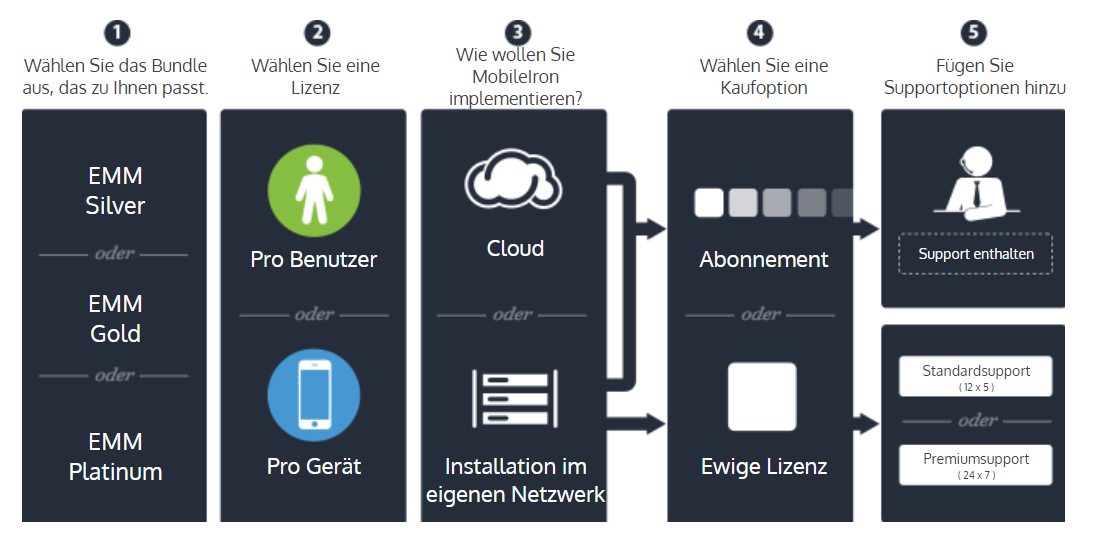
\includegraphics[width=0.95\textwidth]{Bilder/mi_2.png} 
\caption{Mobile Iron Abrechnungsmodell}\label{fig:MobIro2}
\end{figure}

\newpage

% --------------------------------------------------------------------------------------------------------------------------
\section{Samsung Knox}
% --------------------------------------------------------------------------------------------------------------------------

\subsection{Allgemein}\label{sub:Allgemein}
Das weltbekannte Unternehmen Samsung hat ebenfalls an einer Sicherheitslösung für die Mobilnutzung im Unternehmen gearbeitet. Als Produkt ist Samsung Knox, in Anlehnung an Hochsicherheitsstützpunkt Fort Knox, im Portfolio von Samsung zu finden.
Ist man Besitzer aktueller Samsung-Geräten findet man die Applikation \textit{Sicherer Ordner}\footnote{Sicherer Ordner löste am 19. Dezember 2017 den Vorgänger MyKnox ab \cite{sam2017b} }als vorinstallierte Standardsoftware vor. Mit Öffnen dieser App können, nach Eingabe eines benutzerdefinierten Sicherheitsverfahren, verschiedene Einstellungen getätigt werden. Es ist möglich Dateien oder Apps in diesen \flqq sicheren Ordner\frqq  zu verschieben. Sogar Apps die vorher nicht auf dem Smartphone vorhanden sind, können direkt vom Store geladen und installiert werden.Theoretisch wäre dieser Lösungsansatz genau richtig für die Verwendung von BYOD und zusätzlich sogar kostenlos. Dennoch wäre dies nicht umsetzbar im Enterprise-Umfeld.

Um den Anforderungen an eine BYOD-Lösung der Loco AG gerecht zu werden, benötigt es eine MDM-Möglichkeit. Dafür muss die IT-Administration, die Möglichkeit haben die eingesetzten Geräte zu verwalten und somit an die firmeninternen Sicherheitsanforderungen anzupassen. Eine mögliche Lösung bietet Samsung mit der kostenpflichtigen Variante Samsung Knox Premium, die im Folgenden nach dem Kriterienkatalog belichtet werden soll. 

\subsection{Knox-Plattform}
Die Knox-Plattform ist die technische Umsetzung in Hardware und Software, welche standardmäßig in aktuellen Samsung-Geräten vorzufinden ist. Das Sicherheitsverfahren der Knox-Plattform besteht, wie in \cref{fig:SamKno1} sichtbar, aus fünf Komponenten.
\begin{figure}[hbt]
\centering
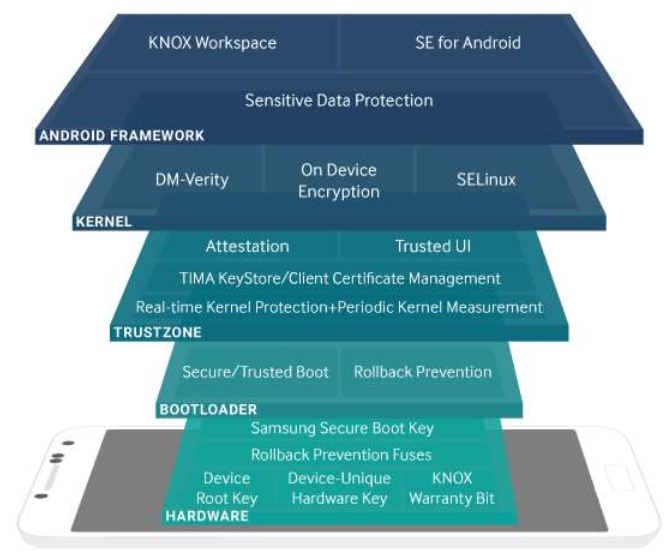
\includegraphics[width=1\textwidth]{Bilder/sk_1}
\caption{Samsung Knox Security Solutions Layers}\label{fig:SamKno1}
\end{figure}
Die Knox-Plattform setzt bereits in der Hardware-Ebene ein. Der Prozessor ist die Steuereinheit auf dem bekanntlich das entsprechende Betriebssystem und die Applikationen laufen. Modi bestimmen welche Priorität, welcher Software oder Applikation zugeschrieben werden. So laufen vom Benutzer installierte Apps im Modus \textit{user mode} und haben somit keinen direkten Zugriff auf die Hardware, das Betriebssystem oder auf andere Apps. Die \textit{ARM TrustZone} beschreibt eine Prozessorarchitektur, die von der Knox-Plattform verwendet wird. Hierbei werden die Modi in \textit{Worlds} eingeteilt. Zum einen die \textit{Normal World}, auf dem standardmäßig alle installierte Software landet und die \textit{Secure World}, die durch kryptographische Methoden gesichert wird und sich in einer isolierten Hardwareumgebung befindet, und somit für das geschäftliche Nutzen des Smartphones eingesetzt werden soll.\footnote{Vgl. \cite{sam2017c}}

Beim Anschalten eines Gerätes, startet für gewöhnlich die Boot-Chain (zu dt. "Hochfahrkette"), die nacheinander die Softwarekomponenten startet. Zum Ausschließen von Fremd- oder Schadsoftware wird ein \textit{Secure Boot} ausgeführt. Jede Komponente in der Kette prüft die Integrität der vorangehenden Komponente durch Abfrage einer Signatur. Wenn die Verifikation einer Signatur fehlschlägt, also eine mögliche Modifikation stattgefunden ist, wird entweder der weitere Startvorgang verhindert oder es wird der \textit{Knox Warranty Fuse} ausgelöst, welcher prüft ob das Gerät vorher jemals einen unzulässigen Status hatte. Allerdings stößt \textit{Secure Boot} beim Unterscheiden von akzeptierten Versionen an seine Grenzen, da er neue Versionen einer Software direkt als gültig sieht. Hierzu wird der \textit{Trusted Boot} hinzugezogen, welcher beim Durchlaufen der Boot-Chain den Hash der nächsten Komponente in die TrustZone Secure World lädt.\footnote{Vgl. \cite{sam2017d} } Es kann also Software nur genehmigt und gestartet werden, die auch als erlaubt in der TrustZone stehen. Das Unternehmen hat die Kontrolle darüber, welche Versionen von welcher Software, sei es öffentlich zugängliche oder eigenentwickelte Software, verwendet werden sollen. 

Denkbar wäre natürlich, dass während der Laufzeit, also nachdem die Überprüfung auf richtige Software, eine fälschliche Modifikation stattfindet. Um dem entgegenzuwirken nutzt Samsung Knox die \textit{Real-Time Kernel Protection} (RKP) um Veränderungen am Kernel zu verhindern und die \textit{Periodic Kernel Measurements} (PKM) zum periodischen Überprüfen der Integrität des Kernels.\footnote{Vgl. \cite{sam2017d} }. Diese beiden Sicherheitsverfahren spielen sich ebenfalls in der \textit{TrustZone Secure World} ab und sind somit isoliert und nicht zugänglich vom Kernel.
Weitere integrierte Verfahren in die Knox-Plattform sind Google DM Verify, genauer beschrieben in \cite{Goo2017a}, welches überprüft ob das Gerät sich im selben Zustand befindet, wie beim letzten Start und SE for Android, genauer beschrieben in \cite{Goo2017b}, dass \textit{mandatory access control} (MAC) über alle Prozesse vollzieht.
\subsection{Knox Solutions}
\subsubsection{Knox Configure}

\subsubsection{Knox Mobile Enrollment}
Um ein EMM-System aufzubauen, ist es notwendig, dass die Mitarbeiter auch Samsung Knox auf ihrem Endgerät installiert haben. Dies findet häufig per Download vom \textit{Google Play store} statt, dem darauf folgenden Authentifizieren und weiteren Einstellen des Workspaces auf die Unternehmensrichtlinien. 
Damit diese manuelle Installation durch den Mitarbeiter vermieden und damit Fehler vermieden werden können, gibt es das \textit{Knox Mobile Enrollment} (KME). Ein Enrollment durch KME funktioniert durch einen Link, der je nach Unternehmensbelangen, bspw. per E-Mail oder Interner Webseite an den Mitarbeiter vermittelt wird. Nachdem dieser Link aufgerufen wird, werden nach entsprechenden Authentifizierungsmaßnahmen, alle Einstellungen und Applikationen automatisch konfiguriert.

\subsubsection{Knox Manage}

\subsubsection{Knox Workspace}
Samsungs Knox Workspace entspricht dem in \cref{sub:Allgemein} beschriebenen \flqq sicheren Ordner\frqq in der Enterprise-Welt. Das heißt, es existiert eine Containerlösung für Mobilgeräte, ersichtlich in \cref{fig:SamKno2}, auf dem geschäftliche Applikationen und Daten von den eigenen getrennt werden können. Es ist nicht möglich außerhalb des Workspaces auf Daten oder Applikationen innerhalb zuzugreifen, aber von innerhalb auf außerhalb. So ist es beispielsweise nicht möglich Bilder, die innerhalb des Workspaces gemacht wurden, außerhalb in der App Galerie anzuschauen.
\begin{figure}[hbt]
\centering
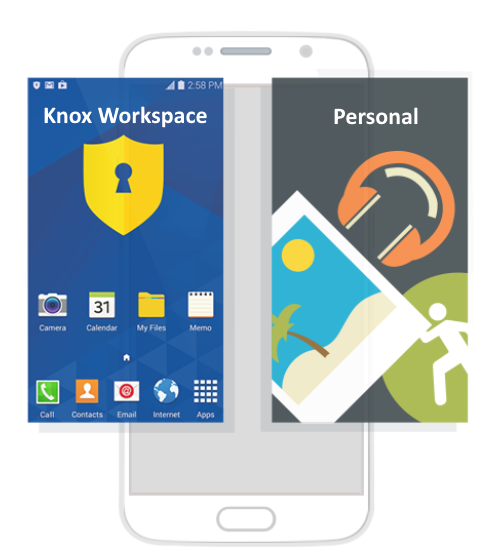
\includegraphics[width=0.5\textwidth]{Bilder/sk_2}
\caption{Samsung Workspace Container}\label{fig:SamKno2}
\end{figure}

Um die Container des Samsungs Workspace zu verwalten, wird das \textit{Mobile Container Management} verwendet. Hierbei können Authentifizierungsmöglichkeiten, Datensicherheit,  VPN, Blacklisting und viele weitere Features, die wie andere EMM Lösungen nutzen gemanagt werden.

Um Zugang zum Workspace zu bekommen wird ein doppeltes Authentifizierungsverfahren verwendet. Hierzu muss der Nutzer zuerst den Fingerabdruck oder wenn es das Gerät zulässt, den Iris-Scanner nutzen und als zweites PIN oder Password eingeben. Erst dann ist ihm Zugriff gewährt.
Andersrum ist es so möglich den Workplace als Authentifizierung zu nutzen. Hierzu gibt es beispielsweise die Möglichkeit per \textit{Near Field Communication} (NFC) das Smartphone als SmartCard agieren zu lassen und so beispielsweise den Zugriff in Sicherheitsbereiche oder Accounts zu gewähren.
Welche Methodiken schlussendlich, wie genutzt werden sollen, kann das IT Management des MCM's je nach Sicherheitsanforderung im Unternehmen anpassen.

\subsubsection{Samsung E-FOTA}
Mit der Samsung E-FOTA-Lösung können alle Geräte mit demselben Betriebssystem betrieben werden.


\subsection{Kompatibilität}
Um Knox Workspace, Knox Mobile Enrollment und Samsung E-FOTA zu nutzen benötigt es eine geeignete EMM-Lösung. In \cref{fig:SamKno3} sind einige EMM Lösungen und deren Kompatibilität mit den Samsung Knox Paketen aufgezeigt.
\begin{figure}[hbt]
\centering
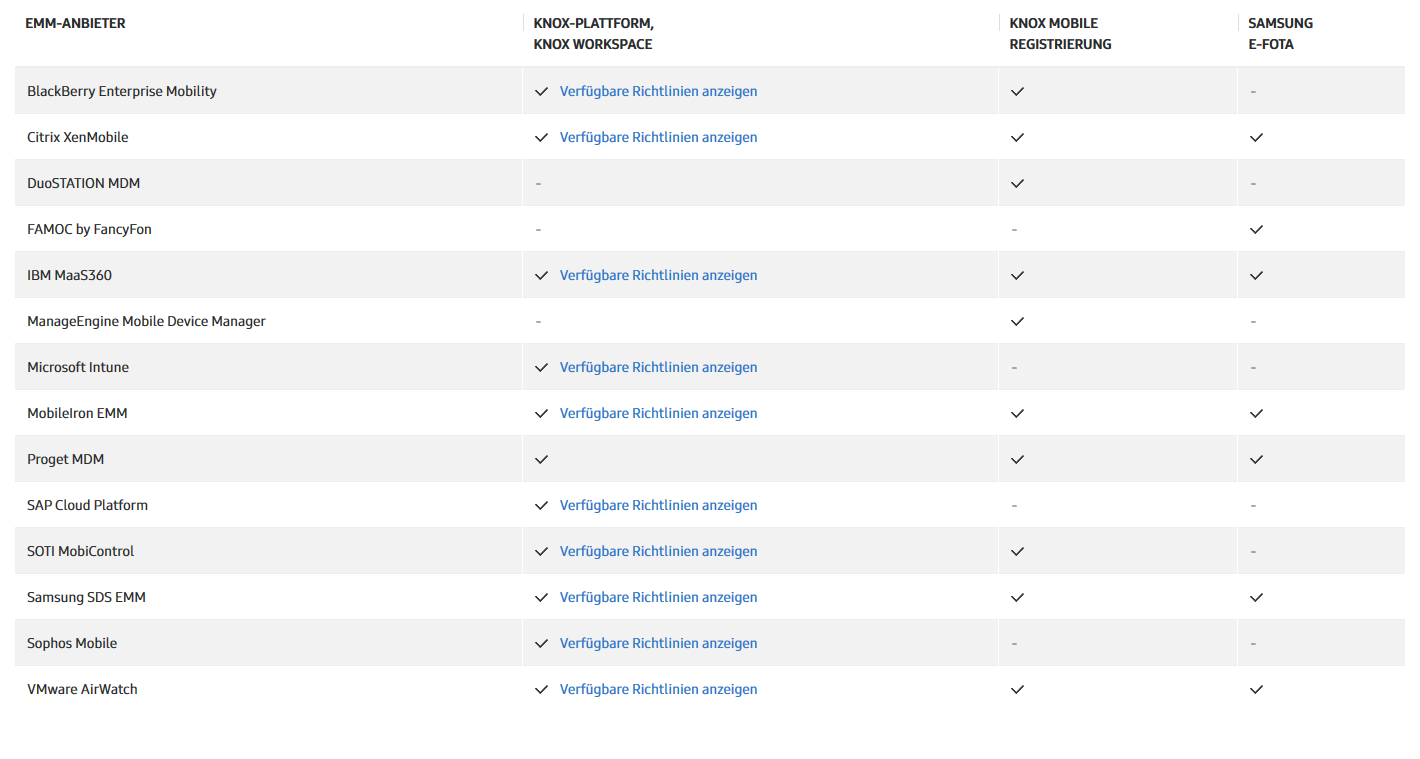
\includegraphics[width=1\textwidth]{Bilder/sk_3}
\caption{Unterstützte EMM-Dienstleister}\label{fig:SamKno3}
\end{figure}

\subsection{Kosten}

\newpage

% --------------------------------------------------------------------------------------------------------------------------
\section{VM AirWatch}
% --------------------------------------------------------------------------------------------------------------------------
\subsection{Paketmodelle}


\subsection{Workspace ONE}
Vmware Workspace ONE ist eine Enterprise-Plattform, die einen digitalen Workspace zu den entsprechenden und geforderten Bedürfnissen bietet. Dieser bietet dem Nutzer 

\subsection{Workspace Horizon}

\subsection{Kosten}
\begin{figure}[hbt]
\centering
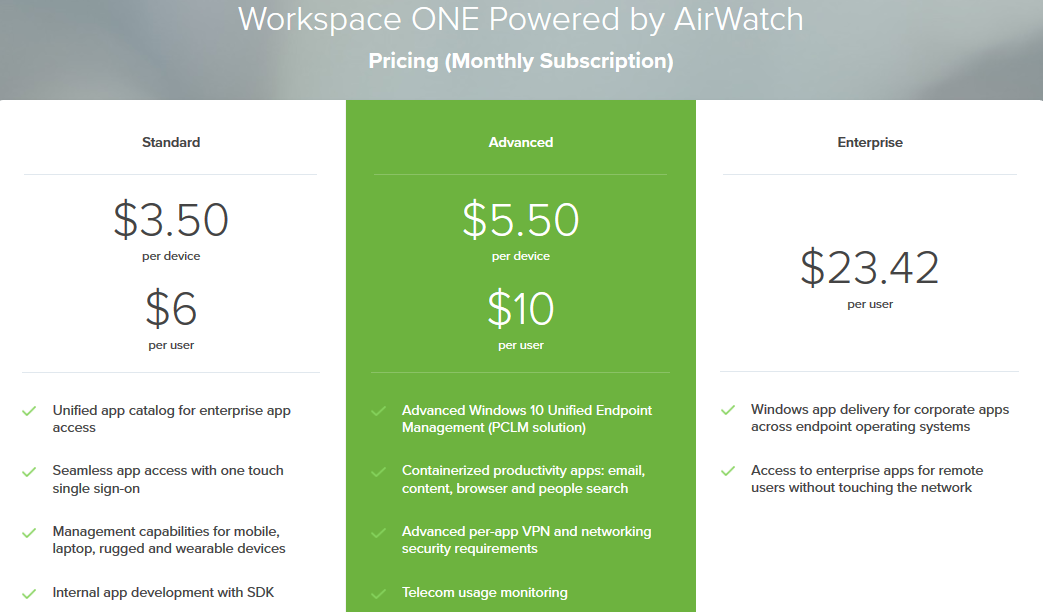
\includegraphics[width=0.95\textwidth]{Bilder/aw_1.png} 
\caption{AirWatch Kosten nach Paket}\label{fig:AirWat1}
\end{figure}
























%\chapter{Vorlagen}
\label{cha:Vorlagen}

\section{Standards}
\subsection{Listenumgebungen und Fußnoten}
Jede wissenschaftliche Arbeit ist natürlich auf Fußnoten\footnote{das sind die kleinen zusätzlichen Hinweise am unteren Rand der Seite} angewiesen. Zudem kommt es immer wieder vor, dass man \marginpar{Bemerkung!}
\begin{itemize}
\item[-] Aufzählungen
\item[+] Nummerierungen oder
\item[*] Definitionen 
\end{itemize}
verwenden muss. In einer Aufzählung \footnote{also in einer \textit{enumerate}-Umgebung} würde das dann so aussehen.
\begin{enumerate}
\item Aufzählungen
\item Nummerierungen oder
\item Definitionen 
\end{enumerate}

In einer Definition \footnote{also in einer \textit{description}-Umgebung} sähe das dann wohl eher so aus:

\begin{description}
\item[Silvester]Jahresendfeier mit Feuerwerk und Alkoholgenuss
\item[Böller] Fuerwerkszubehör ohne visuellen Reiz, dafür aber recht laut
\end{description}
\subsection{Verweise und Zitate}
Natürlich muss man hin und wieder auch auf andere Kapitel verweisen so \zB in diesem Fall auf das Kapitel \ref{cha:wortberge} auf Seite \pageref{cha:wortberge}. Dazu muss das entsprechende Kapitel zuvor entsprechend mit dem Befehl \textit{\bs label\{Labelbezeichner\}} versehen worden sein. In \cite{foobar2003} wird dieser Fall bis ins kleinste Detail beschrieben.

% --------------------------------------------------------------------------------------------------------------------------

\section{Verschiedene Umgebungen}
\label{sec:Umgebungen}

\subsection{Einsatz von Programmlistings}
Für die Vorlage wird das paket \textit{listings} verwendet. \\

\begin{lstlisting} [language=PHP, numbers=left, numberstyle=\tiny, numbersep=10pt]
define('PATH_site', dirname(PATH_thisScript).'/');

if (@is_dir(PATH_site.'typo3/sysext/cms/tslib/')) {
        define('PATH_tslib', PATH_site.'typo3/sysext/cms/tslib/');
} elseif (@is_dir(PATH_site.'tslib/')) {
        define('PATH_tslib', PATH_site.'tslib/');
} else {
      
}
\end{lstlisting}

Das Paket \textit{listings} bietet zahlreiche Konfigurationsmöglichkeiten, um die Quellcodedarstellung an die eigenen Wünsche anzupassen. In einer fertig konfigurierten TexLive-Umgebung erfahren Sie mit dem Kommando

\begin{verbatim}
user@client:~> texdoc listings
\end{verbatim}

mehr über die Möglichkeiten des Pakets.

\subsection{Einsatz von Gleitumgebungen}
\subsubsection{Tabellen}

Tabellen selbst werden in der Umgebung \textit{tabular} oder \textit{tabularx}gesetzt. Um die Tabelle zu einem Gleitobjekt zu machen, muss diese dann in die Umgebung \textit{table} gesetzt werden. 

\begin{table}[hbt]
\centering
\begin{tabular}{c|c|c}
\hline Diese & Tabelle & ist \\ 
\hline zentriert & und  & verwendet \\ 
\hline vertikale & Trennzeichen &  .\\ 
\hline 
\end{tabular}
\caption{Beispiel für eine Tabelle} 

\end{table}


\subsubsection{Bilder}

Bilder werden mit dem Befehl \textit{\bs includecraphics} eingebunden. Um ein Bild zu einem Gleitobjekt zu machen, muss es in die Umgebung figure gesetzt werden.

\begin{figure}[hbt]
\centering

\includegraphics[scale=2.0]{Bilder/logo_dhbw}
\caption{Das Logo der DHBW Karlsruhe}
\end{figure}

Weit hinten, hinter den Wortbergen, fern der Länder Vokalien und Konsonantien leben die Blindtexte. Abgeschieden wohnen Sie in Buchstabhausen an der Küste des Semantik, eines grossen Sprachozeans. Ein kleines Bächlein namens Duden fliesst durch ihren Ort und versorgt sie mit den nötigen Regelialien.

Es ist ein paradiesmatisches Land, in dem einem gebratene Satzteile in den Mund fliegen. Nicht einmal von der allmächtigen Interpunktion werden die Blindtexte beherrscht - ein geradezu unorthographisches Leben.

Eines Tages aber beschloss eine kleine Zeile Blindtext, ihr Name war Lorem Ipsum, hinaus zu gehen in die weite Grammatik. Der grosse Oxmox riet ihr davon ab, da es dort wimmele von bösen Kommata, wilden Fragezeichen und hinterhältigen Semikoli, doch das Blindtextchen liess sich nicht beirren. Es packte seine sieben Versalien, schob sich sein Initial in den Gürtel und machte sich auf den Weg.

Als es die ersten Hügel des Kursivgebirges erklommen hatte, warf es einen letzten Blick zurück auf die Skyline seiner Heimatstadt Buchstabhausen, die Headline von Alphabetdorf und die Subline seiner eigenen Strasse, der Zeilengasse. Wehmütig lief ihm eine rethorische Frage über die Wange, dann setzte es seinen Weg fort.

Unterwegs traf es eine Copy. Die Copy warnte das Blindtextchen, da, wo sie herkäme wäre sie zigmal umgeschrieben worden und alles, was von ihrem Ursprung noch übrig wäre, sei das Wort "und" und das Blindtextchen solle umkehren und wieder in sein eigenes, sicheres Land zurückkehren.




%\chapter{Weit hinter den Wortbergen}
\label{cha:wortberge}


Weit hinten, hinter den Wortbergen, fern der Länder Vokalien und Konsonantien leben die Blindtexte. Abgeschieden wohnen Sie in Buchstabhausen an der Küste des Semantik, eines grossen Sprachozeans. Ein kleines Bächlein namens Duden fliesst durch ihren Ort und versorgt sie mit den nötigen Regelialien.

Es ist ein paradiesmatisches Land, in dem einem gebratene Satzteile in den Mund fliegen. Nicht einmal von der allmächtigen Interpunktion werden die Blindtexte beherrscht - ein geradezu unorthographisches Leben.

Eines Tages aber beschloss eine kleine Zeile Blindtext, ihr Name war Lorem Ipsum, hinaus zu gehen in die weite Grammatik. Der grosse Oxmox riet ihr davon ab, da es dort wimmele von bösen Kommata, wilden Fragezeichen und hinterhältigen Semikoli, doch das Blindtextchen liess sich nicht beirren. Es packte seine sieben Versalien, schob sich sein Initial in den Gürtel und machte sich auf den Weg.

Als es die ersten Hügel des Kursivgebirges erklommen hatte, warf es einen letzten Blick zurück auf die Skyline seiner Heimatstadt Buchstabhausen, die Headline von Alphabetdorf und die Subline seiner eigenen Strasse, der Zeilengasse. Wehmütig lief ihm eine rethorische Frage über die Wange, dann setzte es seinen Weg fort.

Unterwegs traf es eine Copy. Die Copy warnte das Blindtextchen, da, wo sie herkäme wäre sie zigmal umgeschrieben worden und alles, was von ihrem Ursprung noch übrig wäre, sei das Wort "und" und das Blindtextchen solle umkehren und wieder in sein eigenes, sicheres Land zurückkehren.

Doch alles Gutzureden konnte es nicht überzeugen und so dauerte es nicht lange, bis ihm ein paar heimtückische Werbetexter auflauerten, es mit Longe und Parole betrunken machten und es dann in ihre Agentur schleppten, wo sie es für ihre Projekte wieder und wieder missbrauchten.

Und wenn es nicht umgeschrieben wurde, dann benutzen Sie es immer noch.


\textbf{}
%\begin{figure}[htb]
%\centering
%\includegraphics[width=0.8\textwidth]{FHWTLogo.jpg}
%\caption{Das Logo der FHWT}
%\label{fig:FHWTLogo}
%\end{figure}


\chapter{Zusammenfassung}

\section{}

\section{}


% ---------------------------- Literaturverzeichnis ----------------------------------------------
\begin{thebibliography}{999999}

\bibitem[Sa17a]{sam2017}Samsung: \emph{Samsung Knox: mobile Sicherheit für Ihr Unternehmen},\\2017. S.4
\bibitem[Sa17b]{sam2017b}Samsung: \emph{Mitteilung über die Einstellung von My Knox },\\2017, https://my.samsungknox.com/
\bibitem[Sa17c]{sam2017c}Samsung: \emph{Whitepaper: Samsung Knox Security Solution}.\\2017 S.4
\bibitem[Sa17d]{sam2017d}Samsung: \emph{Whitepaper: Samsung Knox Security Solution}.\\2017. S.14
\bibitem[Sa17e]{sam2017e}Samsung: \emph{Whitepaper: Samsung Knox Security Solution}.\\2017. S.15
\bibitem[Sa18]{sam2018}Samsung: \emph{Unterstützte EMM-Dienstleister}.\\2018. https://www.samsungknox.com/de/it-solutions/supported-mdm-vendors
\bibitem[Go17a]{Goo2017a}Google: \emph{Verified Boot}.\\2017. https://source.android.com/security/verifiedboot/
\bibitem[Go17b]{Goo2017b}Google: \emph{Security-Enhanced Linux in Android}.\\2017. https://source.android.com/security/selinux/
\bibitem[Ai18]{Air2018}VMWare: \emph {Airwatch | FAQ}.\\2018.https://www.air-watch.com/de/faq/


\end{thebibliography}

% ------------------------------- Anhang ---------------------------------------------------------

\begin{appendix}
\clearpage
\pagenumbering{Roman}						% römische Seitenzahlen für Anhang
\end{appendix}


\end{document}
